\documentclass[11pt]{article}
\usepackage[utf8]{inputenc}
\usepackage[margin=1in]{geometry}
\usepackage{natbib}
\bibliographystyle{plain}
\usepackage{amsmath}
\usepackage{amssymb}
\usepackage{comment}
\usepackage{amsthm}
\geometry{a4paper}
\usepackage{graphicx}
\usepackage{booktabs}
\usepackage{array}
\usepackage{paralist}
\usepackage{verbatim}
\usepackage{subfig}
\usepackage{multirow}
\usepackage{rotating}
\usepackage{fancyhdr}
\usepackage{hyperref}
\pagestyle{fancy}
\renewcommand{\headrulewidth}{0pt}
\lhead{}\chead{}\rhead{}
\lfoot{}\cfoot{\thepage}\rfoot{}
\usepackage{sectsty}
\allsectionsfont{\sffamily\mdseries\upshape}
\usepackage{algorithm}
\usepackage{algpseudocode}
\usepackage{fancyvrb}

\title{Taiwanese Bankruptcy Feature Analysis Report}
\date{}
\author{CID : 01853006}
\begin{document}
\maketitle

\section{Introduction}

This report models the Taiwanese Bankruptcy Prediction dataset which can be found from the datasets available at UCI, \cite{taiwanese_bankruptcy_dataset}. This dataset concerns data from the Taiwan Economic Journal from $1999$ to $2009$, and contains $94$ predictor features, and one target feature which represents whether the company is bankrupt or not for the data instance considered. 

\section{Initial Data Analysis}\label{EDA}
\begin{figure}
    \centering
    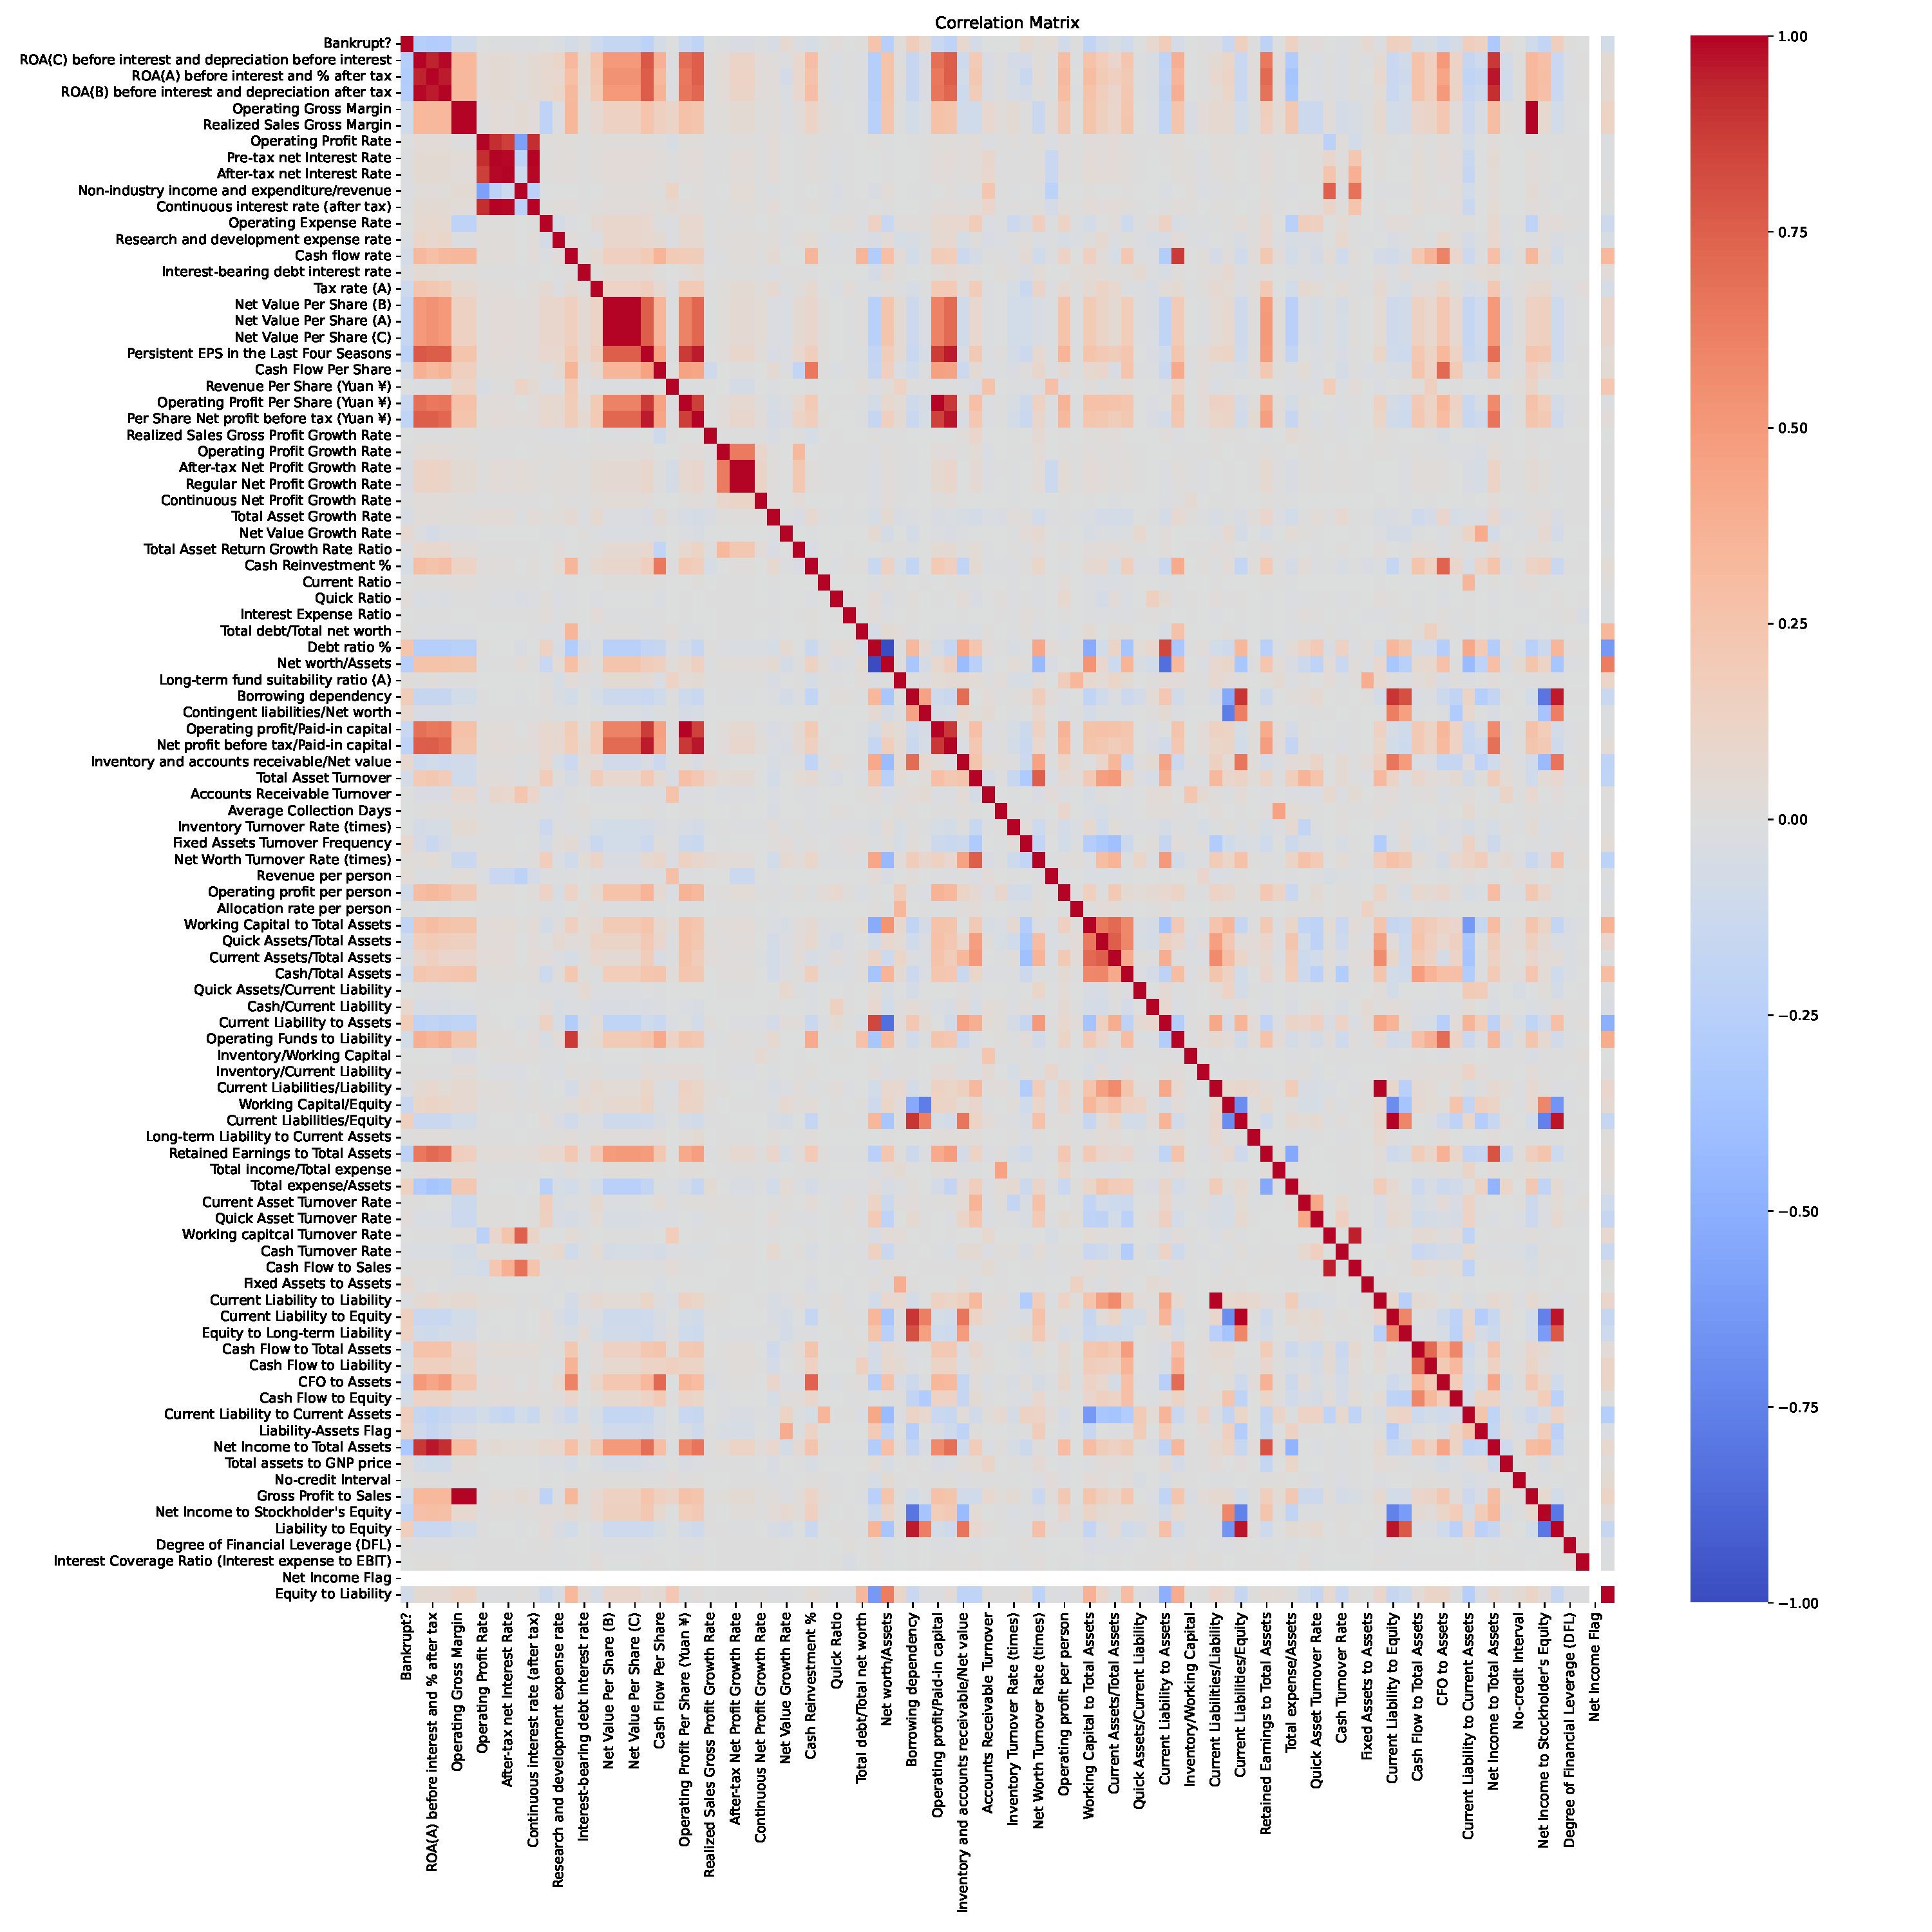
\includegraphics[width = 0.6\textwidth]{correlation_marix.pdf}
    \caption{Heatmap showing correlations}
    \label{fig:CorrelationMatrix}
\end{figure}
This is a relatively large dataset with a large quantity of input variables. As per any modelling, an initial analysis of the data is necessary to get a better understanding of the data which can also help guide the specific path to take with modelling this dataset. \\

A heatmap of correlation between variables can be seen in Figure \ref{fig:CorrelationMatrix}. Whilst the heatmap is not majority a darker shade (indicating high correlation), it is still significant, which can be seen in the upper left quadrant for example. This probes us to further investigate this, and take steps to mitigate this issue of multicolinearity. \\

The analysis also includes checking for missing values and investigating the types of variables that are available in the dataset. One important discovery made about the dataset is that whilst there is a feature called "Net Income Flag", all the datapoints take the same value for this attribute, $1$. This is thus an uninformative variable, and thus is removed. The analysis also revealed that there is one (input) categorical variable called "Liability-Assets Flag", and the rest of the variables are continuous. Acknowledging this helps guide any scaling that needs to be done at a later stage, as different variables have to be handled appropriately appropriately. \\

\begin{figure}
    \centering
    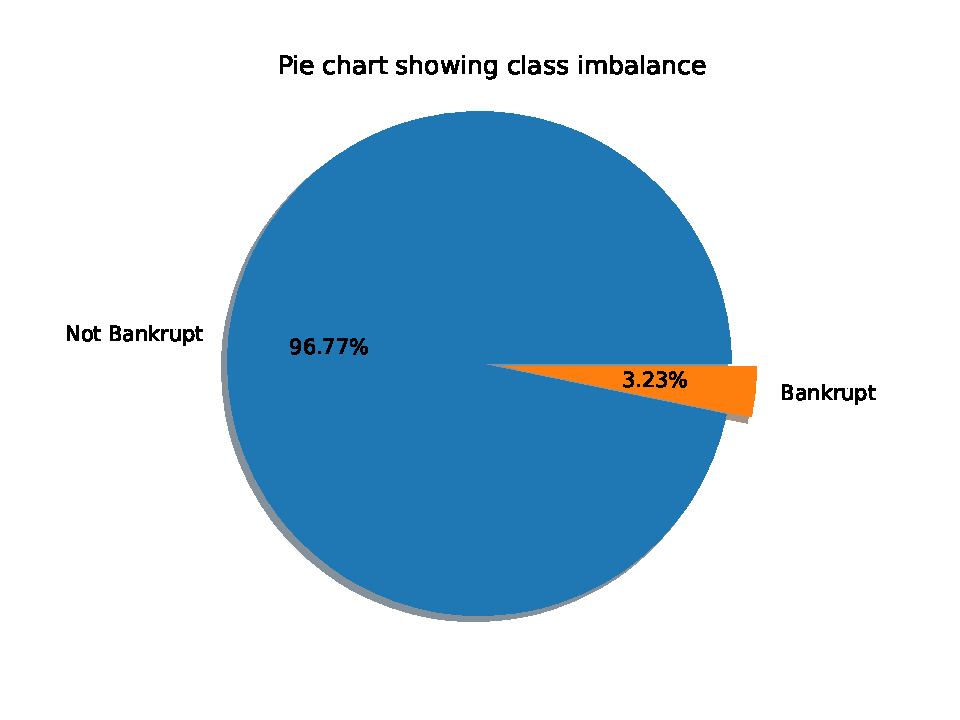
\includegraphics[width=0.5\textwidth]{class_distrib_pie_chart.pdf}
    \caption{Pie chart showing class imbalance}
    \label{fig:ClassImbalance}
\end{figure}
One of the main issues that is observed in this scenario is the extreme class imbalance, as shown in Figure \ref{fig:ClassImbalance}. Measures have to be taken to counter this, as passing this to a machine learning model will cause the model to (heavily) bias the majority class, as opposed to learning meaningful relationships in the data to determine the most appropriate class. This class imbalance also strikes a discussion into the most appropriate metrics to use, as standard classification metric such as accuracy have to be used with great caution, \cite{accuracy_misleading}.

\section{Data Processing}

Common to many machine learning methodologies, a train-test split is created at the start of a project. A stratified split is done as an additional measure to mitigate the class imbalance issue, and ensure that the small number of samples don't all end up in a single set. All feature selection steps or model training/tuning steps are done solely based on the train set, and the test set is held out till the very end. This is to ensure that the model can be fairly evaluated on unseen data, which gives reliable estimates about a model's generalisability. All the feature selection and data processing steps are done using the train dataset as stated. 

As mentioned at the end of Section \ref{EDA}, the dataset suffers from class imbalance which needs to be addressed to appropriately use machine learning models. Techniques such as random under and over sampling form the basis of many advanced techniques such as SMOTE(Synthetic Minority Over-Sampling Technique) \cite{smote}. Under-sampling involves removing data corresponding to the majority class, in attempts to even out the class imbalance, and over-sampling adds data by resampling data from the minority class. Under-sampling causes a loss of data which is not desired, whilst oversampling increases the risk of over-fitting. I perform a mix of under-sampling from the majority class and oversampling from the minority in order to strike a balance between the two approaches. This was done such that the final train dataset had an even class split ($890$ of each class). Whilst \cite{under_over_sampling} achieves better results with over-sampling, since the discrepancy between the majority and minority class is large in our scenario, I opted for a combination of the two in order to not obtain too many duplicate samples via oversampling. The test set is left as it is, without any sampling done to it.\\

As seen in section \ref{EDA}, there is a binary input variable present in the dataset, and the rest are continuous variables. The continuous variables are on different scales, which can pose an issue to a model's ability to learn effectively, since the larger scale may dominate learning, regardless of its true impact on the target feature. The continuous variables are each standardised to achieve mean $0$ and unit variance. A note to make here is that the binary variable is excluded from this scaling, and appended back after the continuous variables are scaled. Omitting allows the variable to retain its interpretation, as scaling may results in it taking values other than $\{0,1\}$. The same scaling done on the train set is applied to the test set to avoid any data leakage.\\ 

\section{Feature Selection} \label{FeatureSelection}

Including all $94$ variables will result in models suffering from the curse of dimensionality, which increases not just the computational load of the model but the risk of over-fitting. To be able to appropriately analyse a feature's importance in determining a company's bankruptcy status, the model should be able to understand and model the underlying relationships within the data, and not just fit to the noise in the data. This is discussed in greater detail in  \cite{feature_selection_curse_of_dim}. \\

To mitigate this issue, I opt for a two-stage filtration process. The first stage is a conducting a Variance Inflation Factor(VIF) analysis. One of the methods to be used in the modelling section, (Section \ref{modelling}) is logistic regression, When using this model, an assumption is made that there is no multicolinearity, which can be violated very easily as seen by the correlation heatmap in Section\ref{EDA}. When two or more variables used are correlated, this is referred to as multicolinearity. Whilst this doesn't impact the models ability to perform prediction, it does cause inflated effects to the model's coefficients. This can cause misleading inference to be done which is an important consideration since our aim is to perform feature importance analysis, which can be done by examining the model coefficients for example. \cite{multicolinearity}, \cite{multicolinearity_midi} discusses this extensively. A VIF score helps detect multicolinearity, and it can be calculated as follows : 
$$
VIF_{i} = \frac{1}{1 - R_i^2} 
$$,
where $R_i^2$ represents the coefficient of determination obtained on the model when the $i^{th}$ predictor variable is used in regression against all the other predictor variables. Literature suggests that scores of above $5$ or $10$ suggest are levels of multicolinearity that should be dealt with. Whilst there are many approaches to deal with this, I opt to remove such variables, and this forms the first stage of the feature selection process. I choose a threshold of $5$ since we have many variables, so we can afford to be on the stricter end of this threshold scale. This narrows the total variables from $94$ to $29$ such variables. These filtered variables are passed to the next and final stage of the feature selection process. \\

The final stage consists of using the filtered variables from VIF to further narrow this down to $20$ variables, which is an appropriate amount of variables to use in regression. Whilst other models are also used in section \ref{modelling} that are not as sensitive to multicolinearity, there must be consistency between all the methods, and thus this process is done. \cite{random_forest_rfe} uses random forest in a recursive elimination process, where a random forest model is fitted, and using the feature importance property of random forests, the unimportant variables, as per the author, is removed before repeating this process on the smaller dataset until desired. Taking inspiration from this but also taking into account the computational complexity of this task, I opt to fit the random forest model once, and then use the top $20$ variables as per the feature importance scores to form the final subset of features to be used. \\

The hyper-parameters are tuned not using cross-validation, but using out of bag (OOB) samples. Random forests trees are fitted using bootstrapped samples, and thus some samples will not be used in fitting the tree. These samples are referred to as the OOB samples, and are used for model evaluation using a score metric that is specified. The choice used here is expanded on later. The model with the hyperparameter configuration that has the best OOB performance is used as the final hyperparameter configuration, and its this model's feature importance attribute that is used. In the case of class imbalance, accuracy of the classifier is a poor choice, since the majority class can be favoured to achieve a good accuracy, as shown in \cite{accuracy_misleading}. The F1 score metric is used, which can be expressed as : 

\begin{equation}
F1 = 2 \times \frac{\text{Precision} \times \text{Recall}}{\text{Precision}+\text{Recall}} 
\label{F1Score}
\end{equation}
where 
$$
\text{Precision} = \frac{TP}{TP+FN} \text{   and   } \text{Recall} = \frac{TP}{TP + FP}
$$
Precision in the context of bankruptcy refers to how many companies that are predicted to be bankrupt are actually bankrupt. High precision would result in the case the when the classifier predicts bankruptcy, its likely this is a correct prediction. Recall refers to how well the classifier in question is able to find all the bankrupt cases. High recall would mean that all companies that are actually bankrupt are detected. This is a very important metric as this shouldn't go missed. Whilst it may seem maximising recall would be best, precision is also of desire, because striking a balance between the two would mean the classifier would be able to understand what makes company bankrupt / not bankrupt. Thus, I opt to maximise the F1 score. The hyperparameter configuration that results in the highest F1 score when evaluated on the OOB samples is chosen as the best performing model. \\

Random forest is used here due to its robustness to class imbalance, which is noted to be an issue for this dataset. Furthermore, a class weight is also used (as supported by sklearn), where weights are adjusted to inversely proportional to the class frequencies, which further helps to mitigate this class imbalance issue. 

\section{Machine Learning Modelling}\label{modelling}
This section gives a brief introduction to the model used, and nuances/choices made when fitting the model.

\begin{figure}
    \centering
    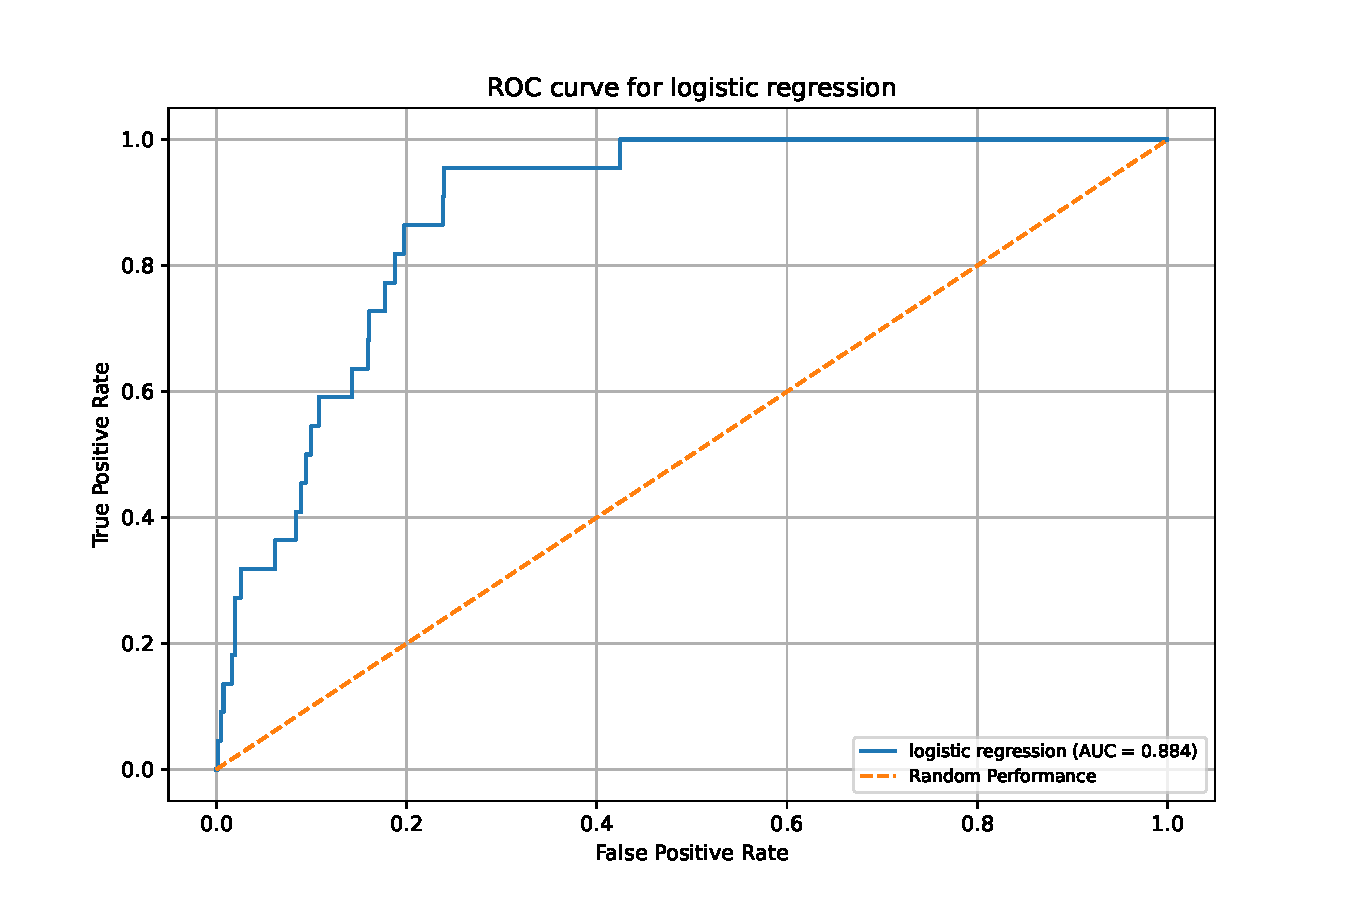
\includegraphics[width = 0.7\textwidth]{logistic_regression_ROC.pdf}
    \caption{ROC curve for logistic regression model}
    \label{fig:logisiticRegressionROC}
\end{figure}

\begin{figure}
    \centering
    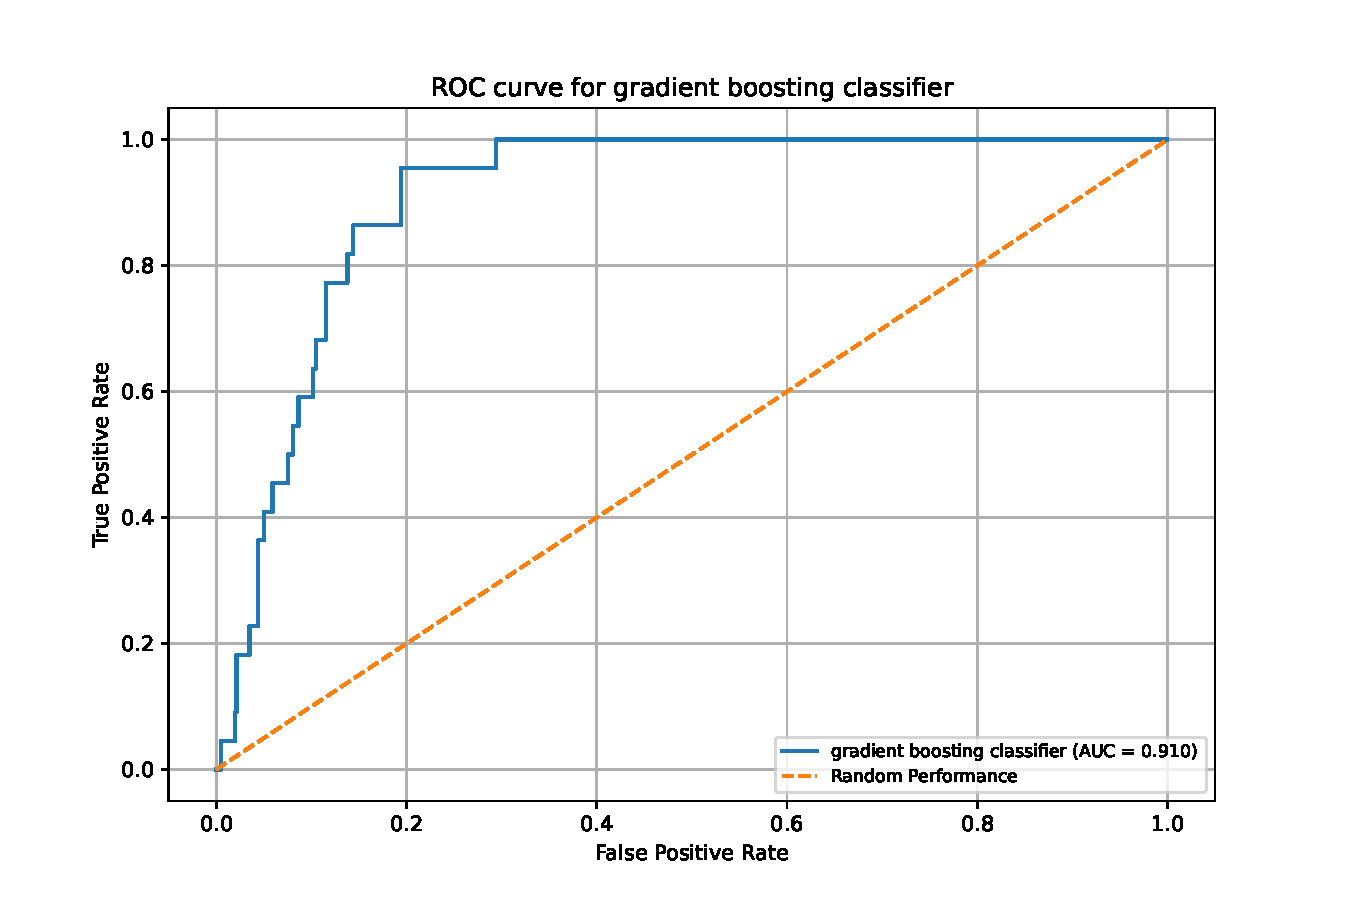
\includegraphics[width = 0.7\textwidth]{gradient_boosting_classifier_ROC.pdf}
    \caption{ROC curve for GBDT model}
    \label{fig:ROC_GDBT}
\end{figure}
\subsection{Logistic Regression}
Linear regression is often chosen due to its inherent simplicity. Whilst standard OLS tries to model the target variable directly, logistic regression uses the sigmoid function to transform into a probability. This allows logistic regression to be useful in classification, and thus why it is included here. \\

A L1 penalty term is used when fitting the logistic regression model, as this penalty term can enforce sparsity in the model. Some of the coefficients can be set to zero, which is important in the realm of feature importance analysis. Using this term comes with the regularization hyper-parameter, that needs to be adequately tuned. To achieve this, cross-validation is used. This can be summarised as splitting the training dataset into $K$ folds ($K$ is set to $10$) and using all but the one fold to train the model, and the left out fold as an evaluation set. This is repeated until every fold is used as the evaluation set once. The best hyper-parameter is chosen such that the F1 score is maximised (Equation \ref{F1Score}).

\subsection{Gradient Boosting Decision Trees}
Gradient boosted decision trees (GBDT) is an ensemble approach where multiple learners are combined together, in a boosting ensemble fashion. A decision tree is constructed, and using the residual error from that tree, the next decision tree is fitted using this error. This sequential steps results in each subsequent learner learning from the previous learner's mistake. To combine the predictions from each, a learning rate is used, and this scale the contribution of the specific tree to the overall prediction. \cite{gbc_paper} uses a gradient boosting classifier for classification albeit in a different context, but still applicable nevertheless. \\

The ROC curve for both of the models, along with the area under the curve score (as part of the legend), show the fit for both, which can be seen in Figure \ref{fig:logisiticRegressionROC} and \ref{fig:ROC_GDBT}. For GDBT, it has a higher AUC score with $0.910$ as opposed to logistic regression's $0.884$. A higher score indicates that the model is better able to separate between the two classes, and this gives us an estimate to how reliable we can think of the model being when performing feature importance analysis. The model having a greater ability to separate the two classes is indication that it has learn useful properties, and thus can interpret the feature importance with more trust.

\section{Model Analysis}
There are many different methods to assess feature importance, which include model-specific approaches such as analysing model coefficients and feature importance property of tree based models, and model-agnostic approaches such as SHAP(SHapley Additive exPlanations) analysis. It is important to note that if one model shows that a particular feature is important, that is not conclusive evidence that is indeed  important. This should be used in combination with the models fitted and other procedures formed, where when a feature is deemed to be important by many models/approaches, it gives us more confidence in the feature's importance in determining the target (bankruptcy). 

\subsection{SHAP Analysis Introduction}
The theory for this introduction is obtained from the following citation \cite{shap_introduction}, as provided in the lecture notes. SHAP analysis is used to explain the outputs from a model. It uses a game theory approach, treating the features as players in the game and its contribution as a payout. Whilst SHAP value is calculated per data point, the absolute value can be taken and average to obtain a mean absolute shap value. Note that absolute value is taken to account that SHAP can be both positive and negative. This give a global view of the feature's importance in predicting the target variable, and thus can be used as a tool for feature importance analysis. A brief introduction is provided here, and I invite the reader to refer to the citation to get a more detailed understanding.

\subsection{Feature Importance Analysis}

\begin{figure}
    \centering
    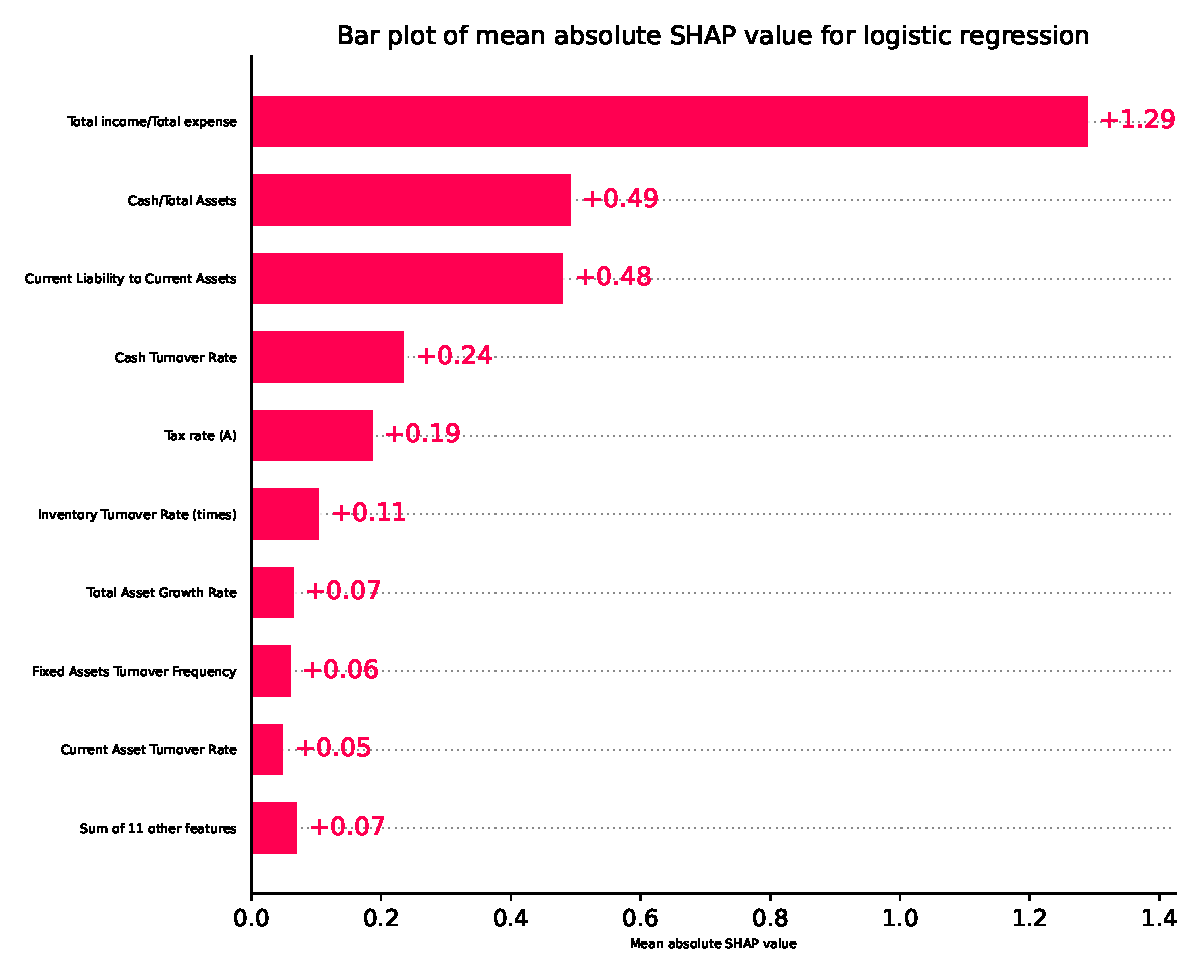
\includegraphics[width=0.6\textwidth]{logistic_regression_SHAP_plot.pdf}
    \caption{Bar plot of the mean absolute SHAP values for Logistic Regression model}
    \label{fig:LogRegSHAP}
\end{figure}

\begin{figure}
    \centering
    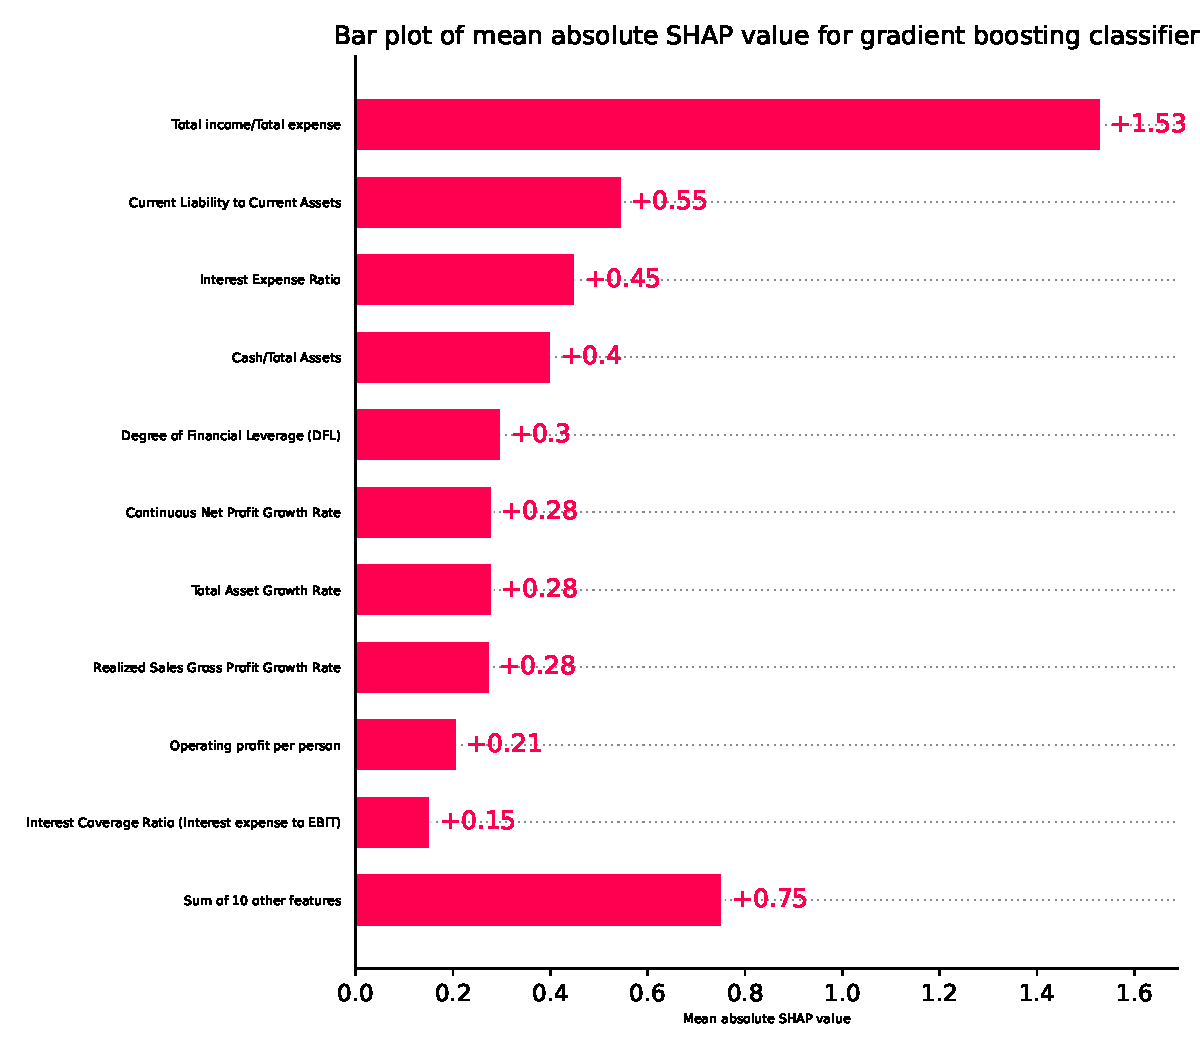
\includegraphics[width=0.6\textwidth]{gradient_boosting_classifier_SHAP_plot.pdf}
    \caption{Bar plot of the mean absolute SHAP values for Gradient Boosting model}
    \label{fig:gbcSHAP}
\end{figure}


\begin{table}[]
    \centering
    \begin{tabular}{|c|c|c|}
    \hline
    Feature Name & LR Coefficient & GBDT Importance Score \\ \hline
       Total income/Total expense & -3.165 & 0.463 \\ \hline
Current Liability to Current Assets & 0.686 & 0.091 \\ \hline
Interest Expense Ratio & 0 & 0.068 \\ \hline
Cash/Total Assets & -0.626 & 0.059 \\ \hline
Interest Coverage Ratio (Interest expense to EBIT) & -0.037 & 0.044 \\ \hline
Degree of Financial Leverage (DFL) & 0.026 & 0.040 \\ \hline
Operating profit per person & -0.020 & 0.039 \\ \hline
Realized Sales Gross Profit Growth Rate & 0.180 & 0.031 \\ \hline
Inventory/Working Capital & 0.072 & 0.030 \\ \hline
Total Asset Growth Rate & 0.079 & 0.029 \\ \hline
Continuous Net Profit Growth Rate & -0.012 & 0.026 \\ \hline
No-credit Interval & 0 & 0.020 \\ \hline
Cash Turnover Rate & -0.251 & 0.018 \\ \hline
Tax rate (A) & -0.234 & 0.011 \\ \hline
Inventory Turnover Rate (times) & -0.111 & 0.007 \\ \hline
Research and development expense rate & -0.037 & 0.006 \\ \hline
Fixed Assets Turnover Frequency & 0.078 & 0.005 \\ \hline
Quick Asset Turnover Rate & 0 & 0.005 \\ \hline
Operating Expense Rate & 0 & 0.004 \\ \hline
Current Asset Turnover Rate & -0.084 & 0.003 \\ \hline
    \end{tabular}
    \caption{Table showing the coefficients from logistic regression (LR) model and the feature importance scores from GBDT}
    \label{tab:modelFeatureImportances}
\end{table}

Figure \ref{fig:LogRegSHAP} and Figure \ref{fig:gbcSHAP} show the mean absolute SHAP value on the test dataset. Comparing these with the coefficients from the logistic regression model and the feature importance scores from gradient boosting classifier, we can obtain a holistic interpretation. The coeffcients for logistic regression and the feature importance scores from GBDT are presented in \ref{tab:modelFeatureImportances}. \\

The logistic regresssion coefficients have an advantage of direct interpretability. That is, the coefficient is the log odds change in the target variable for a unit increase in value taken by the feature, keeping all other features constant. \\

The SHAP values from both models, and the coefficients / feature importance scores from logistic regression all deem that Total Income / Total Expense is the most important factor in determining bankruptcy. This aligns with intuition as if the company is spending more than its income, it only has runway corresponding to their savings since its not making money. One has to note statistical analysis will not take into account economic factors or other factors that may seem currently to be bad, but may provide results in the futures. this includes investments into new divisions etc etc. Other methods have to be incorporated / considered to incorporate this concept of lag, something that isn't considered in this report, but is an extension. We can see that Total Income / Total Expense is clearly a very important feature, as supported by all. Moreover, the magintude of this coefficient for logistic regression is significantly larger than the other features, more than 5x larger than the second most important feature, and for GBDT, the feature is nearly 4x the score of the second most important feature, which further highlights how important the models are deeming this feature to be. The negative logistic regression coefficient indicates that smaller this ratio is, the higher the probability of bankruptcy.  \\

Current liability to current assests is a feature that is deemed to be quite important by both models, both through the inherent feature importance ability but also through the SHAP analysis. This feature is the second most important feature using the coefficient and feature importance score, and third and second most important from the SHAP analysis from loogisic regression and gradient boosting respectively. This shows that this is also another important factor that should be considered in determining a company's bankruptcy status. The logistic regression coefficient is postive, which indicates that a higher such ratio increases the probability of bankruptcy. Considering this is a ratio, this makes sense as  higher ratio would indicate that liabilities are quite high compared to the assets, and thus would indicate high levels of financial stress due to the relative high levels of liability. \\ 

Operating expense rate was a feature whose coefficeint was set to $0$, attributed to the l1 penalty term that encourages this behaviour. Moreover, the GBDT also determined this to be a relatively poor feature, ranking second last in terms of feature importance.  \\

Interest Expense Ratio is an interesting feature since it has coefficient 0 as per logistic regression, but the GBDT score and the SHAP analysis for GBDT deem this to be an important feature, ranking third in mean absolute SHAP value and third in importance scores. The combined interpretation of this is that since logistic regression assumes a linear relationship (in log odds of the target), this shows that the relationship of Interest Expense Ratio is non-linear, and thus the reason why GBDT ranks this highly as it is able to capture such non linear relationships. \\

This analysis shows features such as Total Income / Total Expense is an important feature in determining whether a company will go bankrupt or not, whereas Operating expense rate is not as important, as per the models fitted. The analysis also shows that modelling bankruptcy is quite nuanced, and may involve analysis of a combination of terms / interactions, as seen by the analysis of Interest Expense Ratio. \\

Extensions to this project naturally lead to trying different models and analysisng their respective feature importances. Another possible direction includes considering variables in a wider context and modelling the notion of lag etc. Other extensions is to take a more statistical approach, and use statistical tests to determine significance and importance etc. 

\bibliography{bibliography.bib}
\end{document}
